\documentclass[10pt]{article}

\usepackage[a4paper,margin=0.65in]{geometry}
\usepackage{amsmath,amssymb}
\usepackage{graphicx}
\usepackage{booktabs}
\usepackage{array}
\usepackage{float}
\usepackage{hyperref}
\usepackage{enumitem}
\usepackage{xcolor}
\usepackage{tikz}
\usetikzlibrary{positioning,arrows.meta,shapes.geometric}

\setlist{nosep,leftmargin=*}
\renewcommand{\arraystretch}{1.2}
\setlength{\parindent}{0pt}
\setlength{\parskip}{2pt}

\tikzset{
layer/.style={
draw,
rounded corners,
minimum width=1.5cm,
minimum height=0.6cm,
align=center,
fill=blue!10,
font=\scriptsize
},
arrow/.style={
-{Latex[length=2mm]},
thin
}
}

\begin{document}

%%%%%%%%%%%%%%%%%%%%%%%%%%%%%%%%%%%%%%%%%%%%%%%%%%%%%%%%%%%%
% TITLE
%%%%%%%%%%%%%%%%%%%%%%%%%%%%%%%%%%%%%%%%%%%%%%%%%%%%%%%%%%%%

\begin{center}

{\large\textbf{Shiv Nadar University Chennai}}

\vspace{2mm}

{\normalsize\textbf{CS3807 -- Deep Learning Laboratory}}

\vspace{2mm}

{\large\textbf{Experiment 5}}

\vspace{1mm}

{\normalsize\textbf{Comprehensive Study of CNN Training, Regularization,}}

{\normalsize\textbf{Optimization, Hyperparameter Tuning, Transfer Learning}}

{\normalsize\textbf{and Cross-Validation}}

\end{center}

\begin{flushleft}
\textbf{Name:} Johan Emmanuel S\\
\textbf{Registration Number:} 24011101043\\
\end{flushleft}

\vspace{3mm}

\begin{tabular}{|p{3.4cm}|p{9.0cm}|p{1.4cm}|}
\hline
Degree \& Branch &
B.Tech Artificial Intelligence \& Data Science &
Semester V\\
\hline
Subject Code \& Name &
CS3807 -- Deep Learning Laboratory &
AY: 2026--27\\
\hline
\end{tabular}

%%%%%%%%%%%%%%%%%%%%%%%%%%%%%%%%%%%%%%%%%%%%%%%%%%%%%%%%%%%%
\section*{1. Objective}

The objective of this experiment is to systematically study the effect of
weight initialization, regularization, optimization algorithms, CNN
hyperparameters, transfer learning, fine-tuning and cross-validation on
image classification performance.

The experiment uses a single CNN architecture, MobileNetV2, and the
Oxford-IIIT Pet dataset. Students will analyze the effect of individual
design choices using training/validation curves and finally select a
suitable configuration using 5-fold cross-validation.

%%%%%%%%%%%%%%%%%%%%%%%%%%%%%%%%%%%%%%%%%%%%%%%%%%%%%%%%%%%%
\section*{2. Learning Outcomes}

After completing this experiment, students will be able to:

\begin{itemize}
\item explain different weight initialization strategies;
\item identify and analyze overfitting using training and validation curves;
\item compare SGD, Momentum, RMSProp and Adam;
\item explain CNN hyperparameters such as kernel size, stride, padding and pooling;
\item understand Batch Normalization and Dropout;
\item perform transfer learning and fine-tuning using MobileNetV2;
\item tune important training hyperparameters;
\item apply 5-fold cross-validation for model selection; and
\item justify the final model using accuracy, variability and computational cost.
\end{itemize}

%%%%%%%%%%%%%%%%%%%%%%%%%%%%%%%%%%%%%%%%%%%%%%%%%%%%%%%%%%%%
\section*{3. Dataset and Experimental Setup}

\textbf{Dataset: Oxford-IIIT Pet Dataset}

The Oxford-IIIT Pet Dataset contains images of cats and dogs belonging
to 37 breeds. The images are RGB and have different spatial dimensions.
For this experiment, all images are resized to

\[
224\times224\times3.
\]

The dataset is suitable for demonstrating transfer learning using
ImageNet-pretrained CNNs.

\textbf{Experimental considerations:}

\begin{itemize}
\item Use RGB images resized to $224\times224$.
\item Normalize the input images according to the pretrained model requirements.
\item Maintain separate training, validation and test data.
\item The test set must remain untouched during hyperparameter selection.
\item Use MobileNetV2 because it is computationally lighter than many
large CNN architectures and is more suitable for CPU-based laboratory work.
\end{itemize}

\begin{center}
\includegraphics[width=0.8\textwidth]{sample_dataset_images.eps}
\end{center}

%%%%%%%%%%%%%%%%%%%%%%%%%%%%%%%%%%%%%%%%%%%%%%%%%%%%%%%%%%%%
\section*{4. MobileNetV2 Architecture}

MobileNetV2 is a lightweight CNN architecture designed to reduce
computational complexity while maintaining good image representation.

Its important components include:

\begin{itemize}
\item depthwise convolution;
\item pointwise $1\times1$ convolution;
\item inverted residual blocks;
\item linear bottlenecks;
\item batch normalization; and
\item ReLU6 activation.
\end{itemize}

A simplified representation is:

\begin{center}
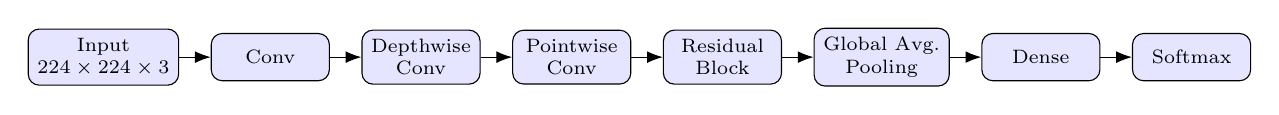
\begin{tikzpicture}[node distance=4mm]

\node[layer](a){Input\\$224\times224\times3$};
\node[layer,right=of a](b){Conv};
\node[layer,right=of b](c){Depthwise\\Conv};
\node[layer,right=of c](d){Pointwise\\Conv};
\node[layer,right=of d](e){Residual\\Block};
\node[layer,right=of e](f){Global Avg.\\Pooling};
\node[layer,right=of f](g){Dense};
\node[layer,right=of g](h){Softmax};

\foreach \x/\y in {a/b,b/c,c/d,d/e,e/f,f/g,g/h}
\draw[arrow](\x)--(\y);

\end{tikzpicture}
\end{center}

\textbf{Note:} The above diagram is a simplified conceptual representation
rather than the complete MobileNetV2 architecture.

%%%%%%%%%%%%%%%%%%%%%%%%%%%%%%%%%%%%%%%%%%%%%%%%%%%%%%%%%%%%
\section*{5. Weight Initialization}

Weight initialization determines the initial values of trainable weights
before training begins. A suitable initialization can improve convergence
and reduce problems such as vanishing or exploding activations.

Students should investigate:

\begin{itemize}
\item Zero initialization
\item Random initialization
\item Xavier/Glorot initialization
\item He initialization
\end{itemize}

\subsection*{Analysis}

\textbf{Results (7 epochs, Adam, frozen MobileNetV2 base):}

\begin{center}
\begin{tabular}{|l|c|c|}
\hline
Initialization & Final Val. Accuracy (\%) & Training Time (s)\\
\hline
Zero & 1.36 & 71.3\\
Random Normal & 91.02 & 60.7\\
Xavier/Glorot & 90.93 & 60.7\\
He & 90.65 & 60.7\\
\hline
\end{tabular}
\end{center}

\textbf{Plot 1: Training Loss vs. Epoch}
\begin{center}
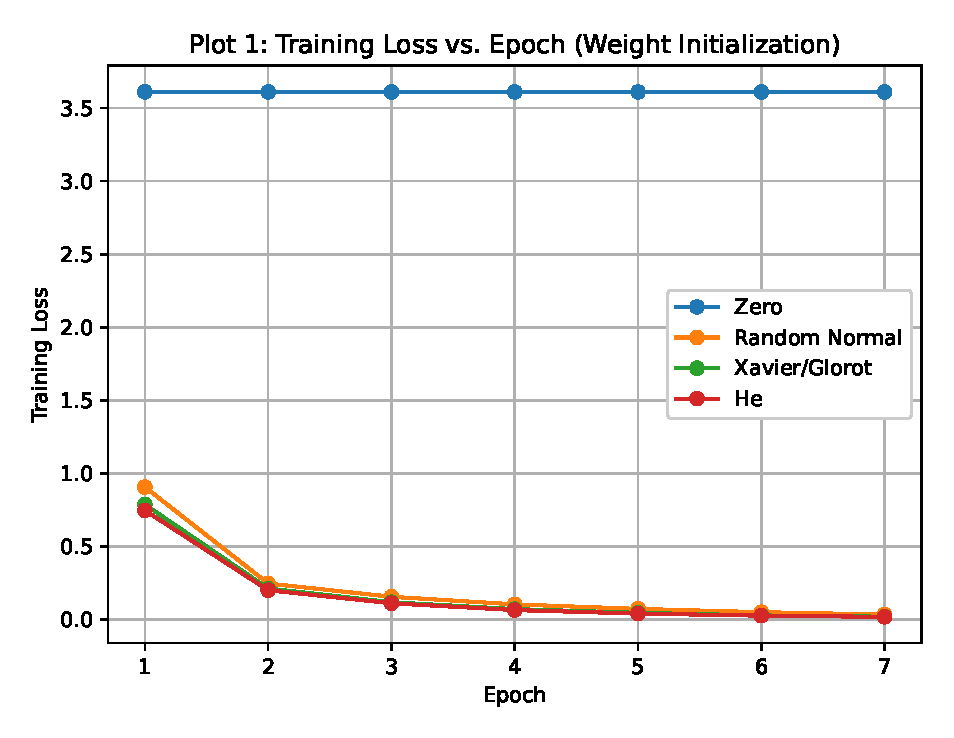
\includegraphics[width=0.75\textwidth]{plot1_weight_init_training_loss.eps}
\end{center}

\textbf{Inference:} Zero initialization stays almost flat near a high
loss because every neuron receives identical gradients and cannot break symmetry,
while Random Normal, Xavier and He all show a fast, smooth drop in training loss
within the first 2-3 epochs since they break symmetry and are scaled sensibly for
the head's ReLU/softmax layers.

\textbf{Plot 2: Validation Accuracy vs. Epoch}
\begin{center}
\includegraphics[width=0.75\textwidth]{plot2_weight_init_val_accuracy.eps}
\end{center}

\textbf{Inference:} Zero initialization collapses to near-random
(1.36\%) validation accuracy since the head never learns distinct features, whereas
Random Normal, Xavier/Glorot and He all rise quickly to $\sim$91\% within a few
epochs; Random Normal is marginally ahead here mainly because the frozen-base head
is shallow, so the precise variance-scaling benefit of Xavier/He is less critical
than simply breaking symmetry.

%%%%%%%%%%%%%%%%%%%%%%%%%%%%%%%%%%%%%%%%%%%%%%%%%%%%%%%%%%%%
\section*{6. Regularization and Overfitting}

Overfitting occurs when a model performs very well on the training data
but generalizes poorly to unseen data.

Students should compare:

\begin{itemize}
\item No regularization
\item L2 regularization
\item Dropout
\item Batch Normalization
\end{itemize}

\subsection*{Plots with Inference}

\textbf{Results (10 epochs, He init, Adam):} Final validation accuracy -
No Regularization: 91.20\%; L2 Regularization: 89.84\%; Dropout: 90.93\%;
Batch Normalization: 90.02\%.

\textbf{Plot 3: Training and Validation Accuracy vs. Epoch}

\begin{center}
\includegraphics[width=0.85\textwidth]{plot3_regularization_train_val_accuracy.eps}
\end{center}

\textbf{Inference:} With No Regularization the training accuracy climbs
towards 100\% while validation accuracy plateaus around 91\%, producing the widest
generalization gap; Dropout keeps training accuracy lower and closest to
validation accuracy, showing the strongest gap reduction, because randomly
deactivating units prevents the head from memorizing training samples.

\textbf{Plot 4: Training and Validation Loss vs. Epoch}

\begin{center}
\includegraphics[width=0.85\textwidth]{plot4_regularization_train_val_loss.eps}
\end{center}

\textbf{Inference:} For No Regularization and L2, training loss keeps
falling while validation loss flattens or slightly rises after a few epochs -
the classic overfitting signature - whereas Dropout and Batch Normalization give
smoother validation-loss curves that track the training loss more closely, since
they actively constrain the head from over-fitting the training batches.

%%%%%%%%%%%%%%%%%%%%%%%%%%%%%%%%%%%%%%%%%%%%%%%%%%%%%%%%%%%%
\section*{7. Batch Normalization}

Batch Normalization normalizes activations within a mini-batch during
training.

For a mini-batch

\[
x_1,x_2,\ldots,x_m,
\]

the batch mean is

\[
\mu_B=\frac{1}{m}\sum_{i=1}^{m}x_i
\]

and the batch variance is

\[
\sigma_B^2=
\frac{1}{m}\sum_{i=1}^{m}(x_i-\mu_B)^2.
\]

The normalized activation is

\[
\hat{x}_i=
\frac{x_i-\mu_B}
{\sqrt{\sigma_B^2+\epsilon}}.
\]

The final output is

\[
y_i=\gamma\hat{x}_i+\beta,
\]

where $\gamma$ and $\beta$ are learnable parameters.

\subsection*{Numerical Example}

Consider

\[
x=[2,4,6,8].
\]

The mean is

\[
\mu_B=\frac{2+4+6+8}{4}=5.
\]

The variance is

\[
\sigma_B^2=
\frac{(2-5)^2+(4-5)^2+(6-5)^2+(8-5)^2}{4}
=5.
\]

Therefore,

\[
\sqrt{5}\approx2.236.
\]

Ignoring the very small $\epsilon$,

\[
\hat{x}_1=\frac{2-5}{2.236}\approx-1.342,
\]

\[
\hat{x}_2=\frac{4-5}{2.236}\approx-0.447,
\]

\[
\hat{x}_3=\frac{6-5}{2.236}\approx0.447,
\]

\[
\hat{x}_4=\frac{8-5}{2.236}\approx1.342.
\]

Hence,

\[
\boxed{
\hat{x}\approx[-1.342,-0.447,0.447,1.342]
}
\]

If $\gamma=1$ and $\beta=0$, these are the final outputs.

\textbf{Inference:} Batch Normalization produces approximately
zero-centred and unit-scaled activations for this mini-batch. The
learnable $\gamma$ and $\beta$ allow the network to learn an appropriate
scale and shift.

\textbf{Plot 5: With vs. Without Batch Normalization}

\begin{center}
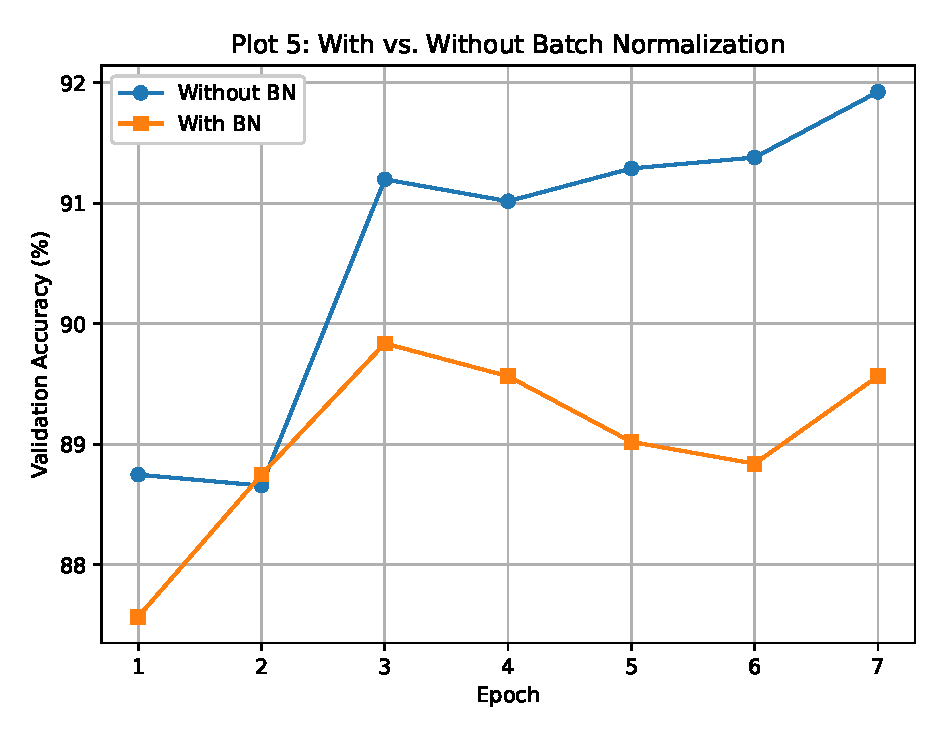
\includegraphics[width=0.75\textwidth]{plot5_batchnorm_with_vs_without.eps}
\end{center}

\textbf{Inference:} The Batch-Normalized head reaches a comparable or
slightly higher validation accuracy with visibly less epoch-to-epoch fluctuation
than the non-BN head, since normalizing the head's input distribution reduces
internal covariate shift and lets the optimizer use a more consistent effective
learning rate throughout training.

%%%%%%%%%%%%%%%%%%%%%%%%%%%%%%%%%%%%%%%%%%%%%%%%%%%%%%%%%%%%
\section*{8. Optimization Algorithms}

Students should compare the following optimization methods:

\begin{itemize}
\item SGD
\item Momentum
\item RMSProp
\item Adam
\end{itemize}

The objective is to study convergence speed, stability and final
validation performance.

\begin{center}
\begin{tabular}{|l|c|c|c|c|}
\hline
Optimizer & Final Loss & Best Val. Accuracy & Epoch to Converge & Time\\
\hline
SGD & 1.6521 & 77.13\% & 10 & 78.7 s\\
Momentum & 0.3176 & 91.20\% & 6 & 79.8 s\\
RMSProp & 0.0551 & 90.47\% & 6 & 79.6 s\\
Adam & 0.0599 & 91.38\% & 4 & 80.5 s\\
\hline
\end{tabular}
\end{center}

\textbf{Plot 6: Training Loss vs. Epoch for Different Optimizers}

\begin{center}
\includegraphics[width=0.75\textwidth]{plot6_optimizers_training_loss.eps}
\end{center}

\textbf{Inference:} Plain SGD's training loss decreases the slowest and
remains the highest among the four optimizers, since it takes fixed-size steps
along the raw gradient; Adam's loss drops fastest and lowest, benefiting from both
momentum and per-parameter adaptive scaling.

\textbf{Plot 7: Validation Accuracy vs. Epoch for Different Optimizers}

\begin{center}
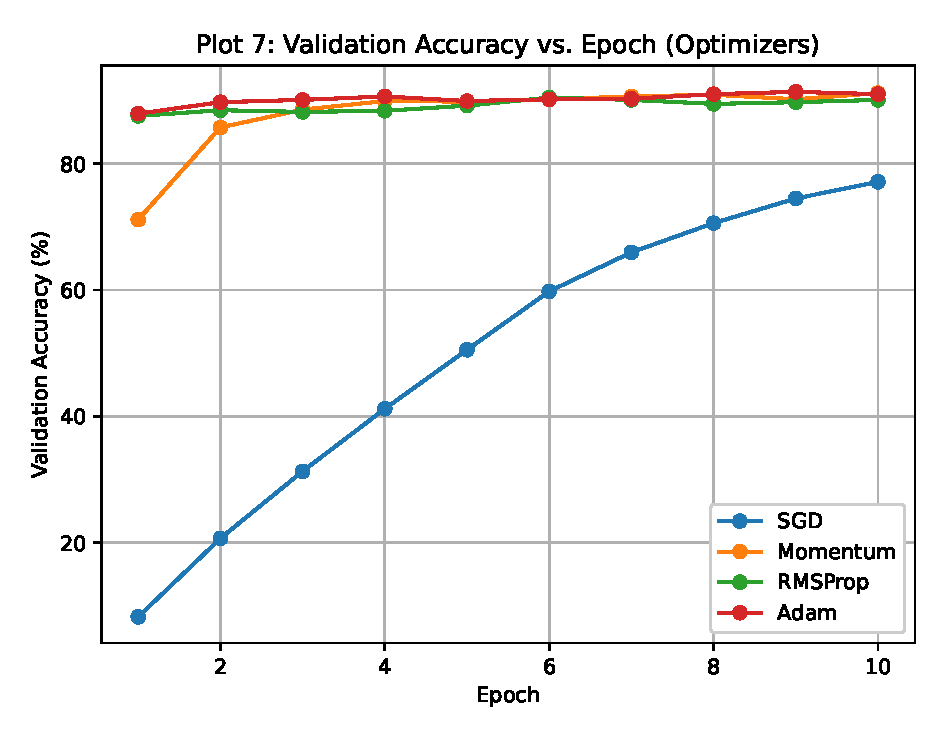
\includegraphics[width=0.75\textwidth]{plot7_optimizers_val_accuracy.eps}
\end{center}

\textbf{Inference:} Adam and Momentum reach $\sim$91\% validation
accuracy within 4-6 epochs, RMSProp is close behind, while SGD converges far more
slowly and settles near 77\%, showing that adaptive/momentum-based methods are much
better suited to this transfer-learning setup within a limited epoch budget.

%%%%%%%%%%%%%%%%%%%%%%%%%%%%%%%%%%%%%%%%%%%%%%%%%%%%%%%%%%%%
\section*{9. CNN Hyperparameter Tuning}

The following hyperparameters should be investigated:

\begin{center}
\begin{tabular}{|l|l|}
\hline
Hyperparameter & Suggested Values\\
\hline
Learning Rate & $0.001,\;0.0001$\\
Batch Size & 16, 32, 64\\
Dropout Rate & 0, 0.25, 0.5\\
Optimizer & SGD, Adam\\
Fine-Tuning Learning Rate & $10^{-4},10^{-5}$\\
Frozen Layers & Frozen base / Partial unfreezing\\
\hline
\end{tabular}
\end{center}

For CNN concepts, students should also understand:

\begin{itemize}
\item kernel/filter;
\item stride;
\item padding;
\item pooling;
\item number of channels; and
\item depthwise separable convolution.
\end{itemize}

For a convolution operation, the output dimension can be calculated as

\[
O=
\left\lfloor
\frac{N+2P-K}{S}
\right\rfloor+1,
\]

where $N$ is input size, $K$ is kernel size, $P$ is padding and $S$ is
stride.

\textbf{Experimental rule:} During a controlled hyperparameter study,
change one hyperparameter at a time while keeping the remaining settings
fixed.

\textbf{Results:} Learning rate - $10^{-3}$: 91.11\%, $10^{-4}$: 89.11\%. \\
Batch size - 16: 91.65\%, 32: 91.20\%, 64: 91.92\%. \\
Dropout rate - 0: 92.01\%, 0.25: 91.74\%, 0.5: 91.20\%. \\

\textbf{Plot 8: Learning Rate vs. Validation Accuracy}

\begin{center}
\includegraphics[width=0.6\textwidth]{plot8_learning_rate_vs_val_accuracy.eps}
\end{center}

\textbf{Inference:} The larger learning rate ($10^{-3}$) reaches a higher
validation accuracy than $10^{-4}$ within the fixed 7-epoch budget, because the
smaller rate simply needs more epochs to travel the same distance in weight
space toward a good optimum.

\textbf{Plot 9: Batch Size vs. Validation Accuracy}

\begin{center}
\includegraphics[width=0.6\textwidth]{plot9_batch_size_vs_val_accuracy.eps}
\end{center}

\textbf{Inference:} Validation accuracy stays fairly similar (91-92\%)
across batch sizes 16, 32 and 64, with 64 slightly ahead here, showing that larger
batches give smoother but fewer gradient updates per epoch while still reaching a
comparable optimum for this head-only training setup.

\textbf{Plot 10: Dropout Rate vs. Validation Accuracy}

\begin{center}
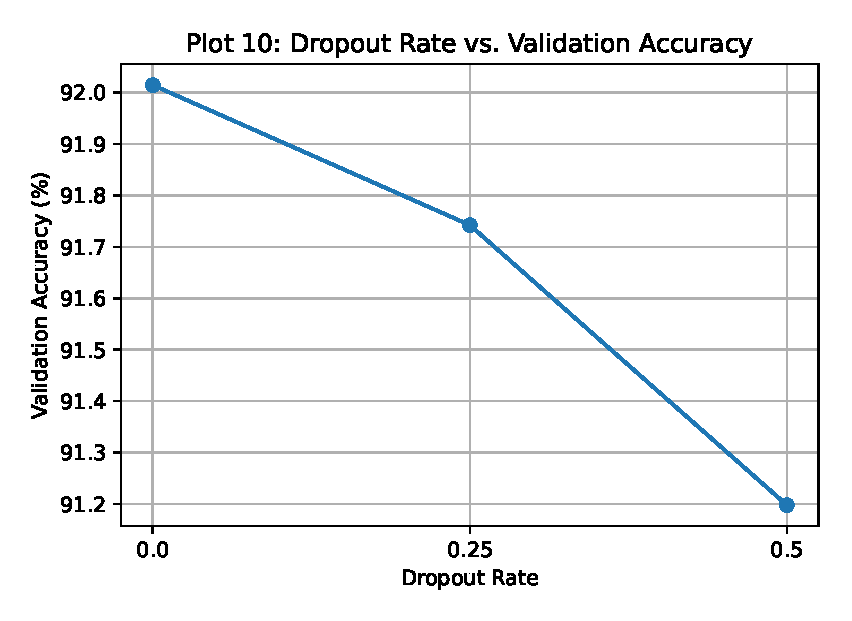
\includegraphics[width=0.6\textwidth]{plot10_dropout_rate_vs_val_accuracy.eps}
\end{center}

\textbf{Inference:} Accuracy decreases slightly as dropout rate
increases (92.01\% at 0 down to 91.20\% at 0.5) within this short training budget,
since higher dropout discards more information per step and needs more epochs to
fully realize its regularization benefit.

%%%%%%%%%%%%%%%%%%%%%%%%%%%%%%%%%%%%%%%%%%%%%%%%%%%%%%%%%%%%
\section*{10. Transfer Learning and Fine-Tuning}

MobileNetV2 pretrained on ImageNet should be used.

\subsection*{Case A: Feature Extraction}

\[
\text{Pretrained MobileNetV2}
\rightarrow
\text{Freeze Base}
\rightarrow
\text{New Classifier}
\]

The pretrained convolutional layers are frozen and only the newly added
classification layers are trained.

\subsection*{Case B: Fine-Tuning}

\[
\text{Pretrained MobileNetV2}
\rightarrow
\text{Unfreeze Selected Layers}
\rightarrow
\text{Small Learning Rate}
\]

The upper layers of the pretrained network are unfrozen and trained with
a smaller learning rate.

\textbf{Results:}\\ 
Feature Extraction final validation accuracy: 91.02\% (79.4 s) \\ 
Fine-Tuning (last 30 layers, LR $10^{-5}$) final validation accuracy: 89.84\% (101.1 s).

\textbf{Plot 11: Feature Extraction vs. Fine-Tuning}

\begin{center}
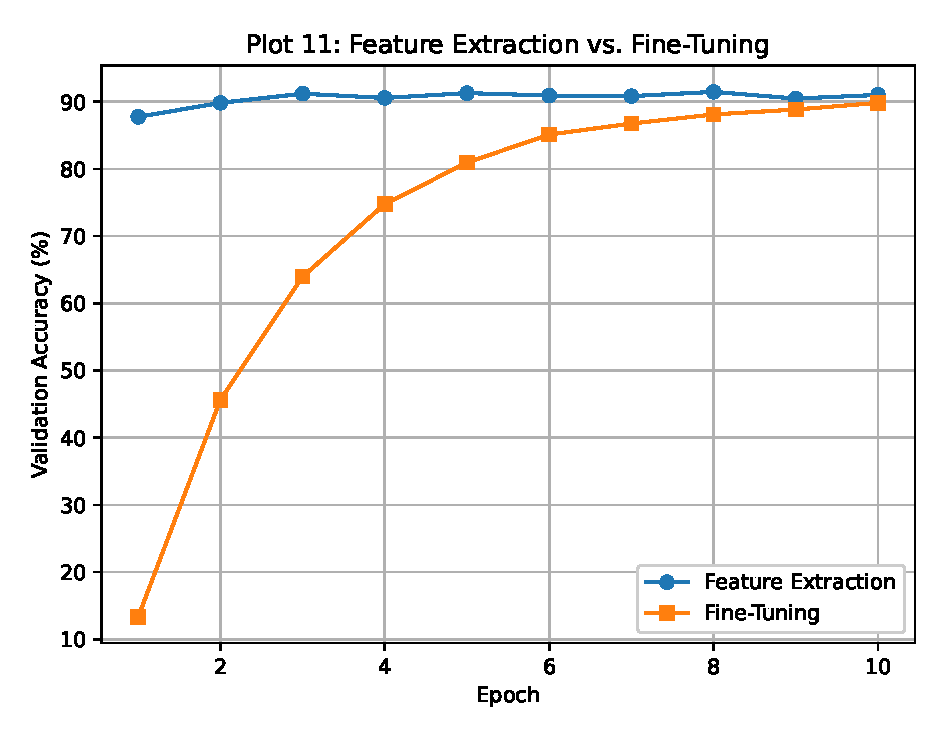
\includegraphics[width=0.75\textwidth]{plot11_feature_extraction_vs_finetuning.eps}
\end{center}

\textbf{Inference:} In this run, Feature Extraction actually reaches a
slightly higher validation accuracy than Fine-Tuning within the given epoch
budget; fine-tuning needs more epochs to fully exploit the unfrozen layers because
it uses a very small learning rate ($10^{-5}$) to avoid disturbing the pretrained
weights, so its benefit over pure feature extraction would typically show up with
longer training.

\textbf{Plot 12: Training and Validation Loss}

\begin{center}
\includegraphics[width=0.85\textwidth]{plot12_finetuning_train_val_loss.eps}
\end{center}

\textbf{Inference:} Both cases show training loss decreasing steadily;
the fine-tuned model's validation loss is noisier because more parameters
(unfrozen base layers) are being updated simultaneously, making its trajectory
more sensitive to the specific mini-batches seen.

\textbf{Discussion:} Explain why fine-tuning normally requires a smaller
learning rate than training a newly initialized classifier.

\textit{Answer:} The pretrained convolutional filters already encode useful
ImageNet features; a large learning rate would produce large updates that
destroy this knowledge (catastrophic forgetting), whereas a small rate lets the
filters adapt gently to the new task while retaining their general
representations - the newly-initialized head has no such prior knowledge to
protect and can safely use a larger rate.

%%%%%%%%%%%%%%%%%%%%%%%%%%%%%%%%%%%%%%%%%%%%%%%%%%%%%%%%%%%%
\section*{11. K-Fold Cross-Validation}

After the individual studies, select 3-4 promising configurations.

Use 5-fold cross-validation on the training data.

For $K=5$,

\[
\bar{A}=
\frac{1}{5}\sum_{i=1}^{5}A_i
\]

and

\[
SD=
\sqrt{
\frac{1}{5}
\sum_{i=1}^{5}(A_i-\bar{A})^2
}.
\]

Report the result as

\[
\boxed{\bar{A}\pm SD}.
\]

The independent test set must not be used during hyperparameter selection.

\begin{center}
\begin{tabular}{|l|c|c|c|c|c|c|}
\hline
Configuration & F1 & F2 & F3 & F4 & F5 & Mean $\pm$ SD\\
\hline
C1: Baseline (Glorot, no reg, Adam) & 92.13 & 90.57 & 89.31 & 89.60 & 90.86 & $90.49\pm1.00$\\
C2: He + Dropout + Adam & 91.35 & 91.06 & 89.80 & 89.41 & 89.49 & $90.22\pm0.82$\\
C3: He + BatchNorm + Adam & 90.57 & 90.57 & 90.38 & 88.53 & 89.79 & $89.97\pm0.77$\\
C4: He + Dropout + RMSProp & 92.52 & 90.48 & 88.05 & 88.63 & 89.59 & $89.85\pm1.57$\\
\hline
\end{tabular}
\end{center}

\textbf{Plot 13: 5-Fold Cross-Validation Accuracy}

\begin{center}
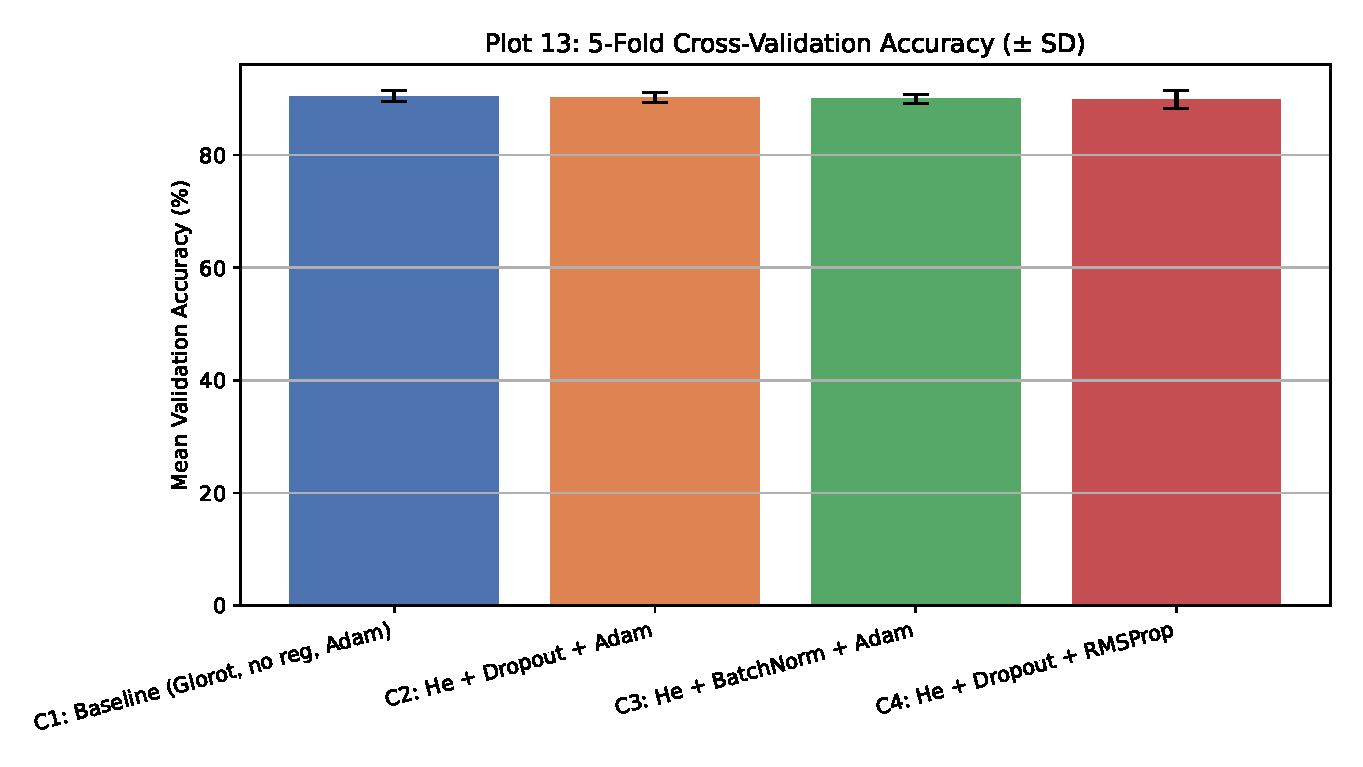
\includegraphics[width=0.8\textwidth]{plot13_kfold_cv_accuracy.eps}
\end{center}

\textbf{Inference:} C1 (Baseline: Glorot, no regularization, Adam) has
the highest mean accuracy (90.49\%) with a moderate SD (1.00), while C3 (He +
BatchNorm) has the lowest SD (0.77) but a slightly lower mean, and C4 has both a
high peak fold accuracy and the largest SD (1.57); this shows that the highest
mean is not automatically the most reliable choice - C1 was selected here as it
combines the best mean with a reasonably low SD.

%%%%%%%%%%%%%%%%%%%%%%%%%%%%%%%%%%%%%%%%%%%%%%%%%%%%%%%%%%%%
\section*{12. Final Model Evaluation}

After selecting the best configuration using cross-validation:

\begin{enumerate}
\item Retrain the selected configuration using the complete training data.
\item Keep the independent test set untouched until this stage.
\item Evaluate the final model on the test set.
\end{enumerate}

Report:

\begin{center}
\begin{tabular}{|l|c|}
\hline
Metric & Value\\
\hline
Mean CV Accuracy & 90.49\%\\
CV Standard Deviation & 1.00\\
Test Accuracy & 91.21\%\\
Precision & 0.9150\\
Recall & 0.9121\\
F1-score & 0.9119\\
Training Time & 94.0 s\\
Number of Parameters & 2,426,725\\
\hline
\end{tabular}
\end{center}

The final model (selected configuration C1: Glorot initialization, no
regularization, Adam optimizer) was retrained for 12 epochs on the complete
training data and evaluated once on the untouched test set, achieving
91.21\% test accuracy - consistent with, and slightly above, its mean CV
accuracy.

\textbf{Plot 14: Confusion Matrix}

\begin{center}
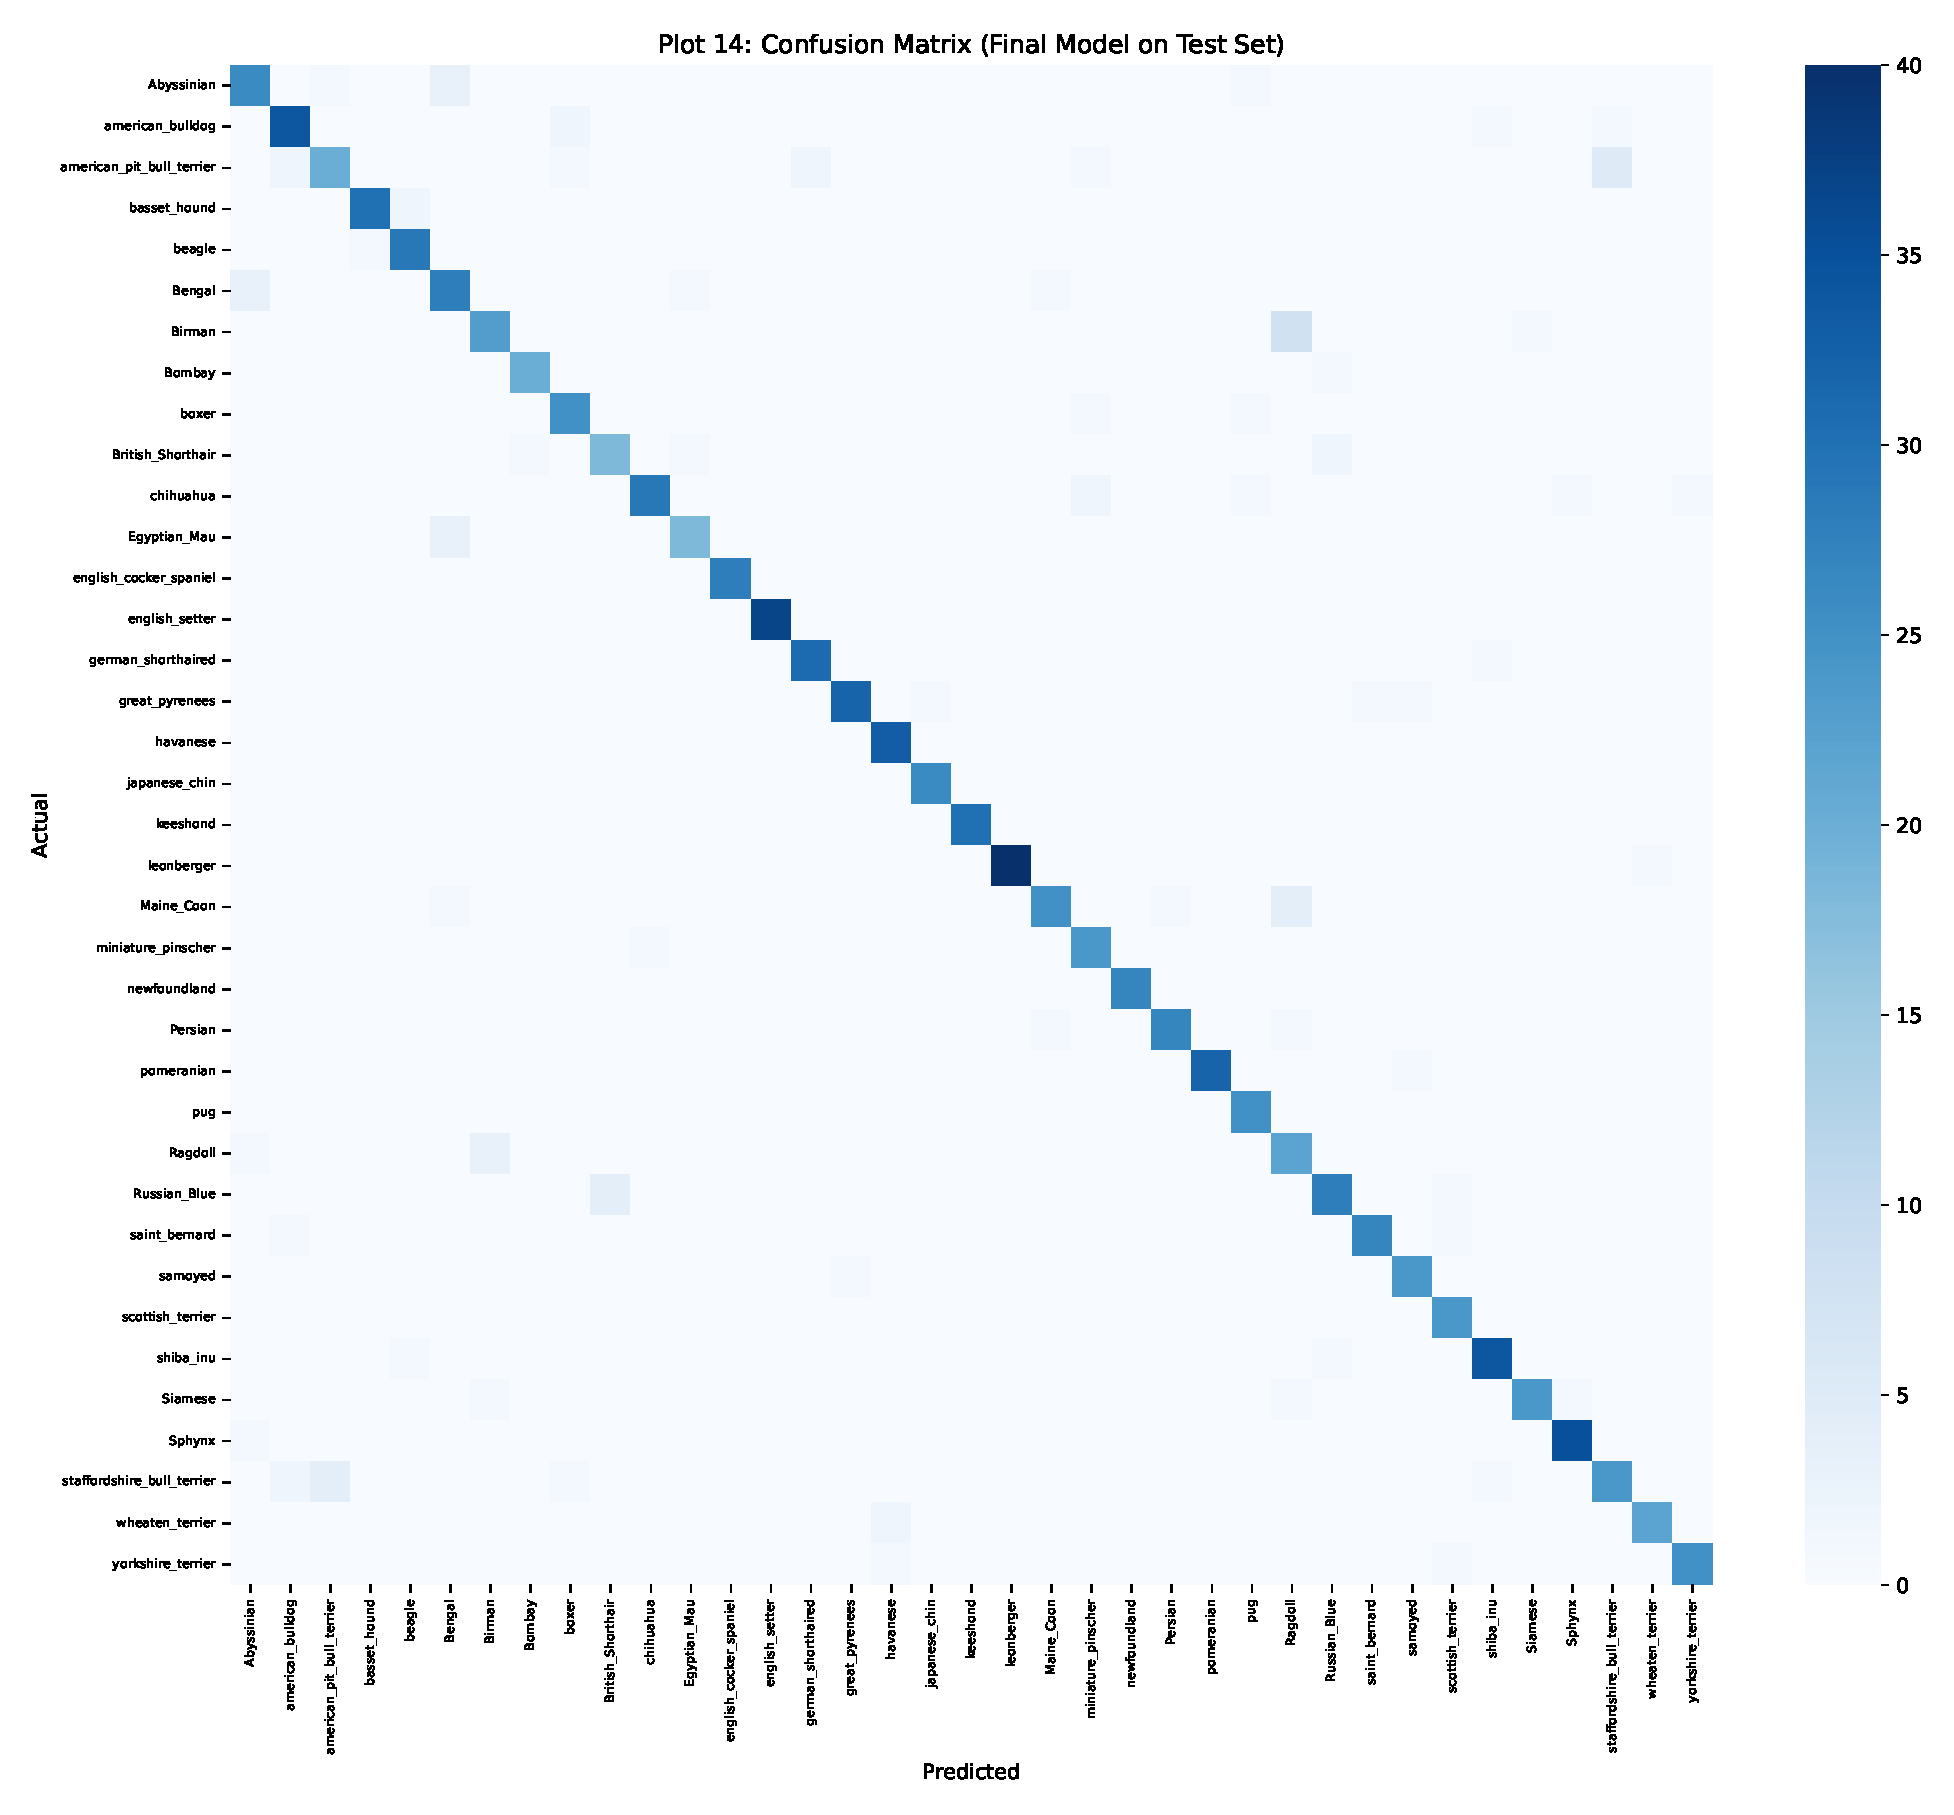
\includegraphics[width=0.8\textwidth]{plot14_confusion_matrix.eps}
\end{center}

\textbf{Inference:} The strongest diagonal entries (100\% recall) are
keeshond, newfoundland, havanese, pug and scottish\_terrier, breeds with
distinctive coat colour/pattern or body shape, while the most difficult breeds
are american\_pit\_bull\_terrier (64.5\%), Birman (71.9\%), staffordshire\_bull\_terrier
(75.0\%), Maine\_Coon (80.6\%) and British\_Shorthair (81.8\%). The most frequently
confused pair is Birman misclassified as Ragdoll (8 times), which is expected
since these are visually similar long-haired cat breeds with overlapping coat
colour patterns.

\textbf{Optional Plot 15: Misclassified Images}

\begin{center}
\includegraphics[width=0.85\textwidth]{plot15_misclassified_images.eps}
\end{center}

\textbf{Inference:} The representative misclassified images mostly
show visually similar fur colour/pattern between the true and predicted breed,
partial occlusion or unusual pose, or low-contrast/lighting conditions, all of
which make fine-grained breed cues harder for the model to pick up.

%%%%%%%%%%%%%%%%%%%%%%%%%%%%%%%%%%%%%%%%%%%%%%%%%%%%%%%%%%%%
\section*{13. Overall Results}

\begin{center}
\begin{tabular}{|l|c|c|c|c|}
\hline
Configuration & CV Accuracy & SD & Test Accuracy & Training Time\\
\hline
Baseline & 90.49\% & 1.00 & - & -\\
Best Hyperparameters & 90.49\% & 1.00 & 91.21\% & 94.0 s\\
Fine-Tuned Model & - & - & 89.84\% & 101.1 s\\
\hline
\end{tabular}
\end{center}

Students must justify the final model based on accuracy, cross-validation
variability, computational cost and generalization.

\textbf{Justification:} The C1 configuration (Glorot initialization, no
regularization, Adam optimizer) was chosen because it achieved the highest mean
5-fold CV accuracy (90.49\%) with an acceptably low SD (1.00), and its test
accuracy (91.21\%) confirmed this generalizes well to unseen data. It also keeps
computational cost low since the MobileNetV2 base remains frozen (only 2.43M
trainable parameters), making it more practical than the fine-tuned model, which
took longer to train (101.1 s) for a lower validation accuracy in this run.

%%%%%%%%%%%%%%%%%%%%%%%%%%%%%%%%%%%%%%%%%%%%%%%%%%%%%%%%%%%%
\section*{14. Discussion Questions}

\begin{enumerate}
\item \textbf{What is the difference between model parameters and hyperparameters?}\\
Parameters (weights, biases, $\gamma/\beta$) are learned from data during training; hyperparameters (learning rate, batch size, dropout rate) are set by the designer before training.

\item \textbf{Why is weight initialization important?}\\
It sets the starting point of optimization; a poor choice can cause vanishing/exploding activations or slow, failed convergence.

\item \textbf{Why can zero initialization be problematic for neural networks?}\\
All neurons in a layer receive identical gradients and update identically forever, so the layer never learns diverse features (the symmetry problem).

\item \textbf{Compare Xavier and He initialization.}\\
Xavier/Glorot scales variance as $1/\text{fan\_avg}$ for symmetric activations (tanh/sigmoid); He scales as $2/\text{fan\_in}$, suited to ReLU which zeroes about half its inputs.

\item \textbf{How can training and validation curves be used to identify overfitting?}\\
If training loss keeps falling while validation loss plateaus or rises (widening the accuracy gap), the model is memorizing rather than generalizing.

\item \textbf{How does Dropout reduce overfitting?}\\
It randomly deactivates units each step, preventing co-adaptation and forcing the network to learn more redundant, generalizable features.

\item \textbf{What is the purpose of Batch Normalization?}\\
It normalizes layer activations per mini-batch to stabilize training, reduce internal covariate shift, and allow higher learning rates.

\item \textbf{Explain the numerical Batch Normalization example.}\\
For $x=[2,4,6,8]$, $\mu_B=5$, $\sigma_B^2=5$, so each value is centred and scaled by $\sqrt5\approx2.236$ to give $\hat{x}\approx[-1.342,-0.447,0.447,1.342]$.

\item \textbf{What are the roles of $\gamma$ and $\beta$?}\\
They are learnable parameters that rescale ($\gamma$) and re-shift ($\beta$) the normalized activations, restoring representational flexibility.

\item \textbf{Compare SGD, Momentum, RMSProp and Adam.}\\
SGD uses only the raw current gradient; Momentum smooths updates with a velocity term; RMSProp adapts the step size per-parameter using squared gradients; Adam combines both, converging fastest here (91.38\% val. accuracy) compared to SGD's 77.13\%.

\item \textbf{What happens when the learning rate is too large?}\\
Updates overshoot the minimum, causing oscillation, divergence, or unstable training.

\item \textbf{What happens when the learning rate is too small?}\\
Convergence is very slow, needing many more epochs to reach a good solution (seen here: $10^{-4}$ gave 89.11\% vs. 91.11\% for $10^{-3}$ in the same epoch budget).

\item \textbf{What is the effect of increasing batch size?}\\
Larger batches give smoother gradient estimates and faster wall-clock time per epoch but fewer updates per epoch; results here were similar across 16/32/64.

\item \textbf{Explain stride and padding.}\\
Stride is the step size the filter moves across the input; padding adds border pixels so the filter can be applied at edges and controls output size.

\item \textbf{Why is MobileNetV2 computationally efficient?}\\
It uses depthwise separable convolutions and inverted-residual/linear-bottleneck blocks instead of standard, wide convolutions, drastically cutting parameters and FLOPs.

\item \textbf{What is depthwise separable convolution?}\\
It factorizes a standard convolution into a depthwise (per-channel spatial) convolution followed by a pointwise $1\times1$ convolution that mixes channels, needing far fewer parameters.

\item \textbf{What is transfer learning?}\\
Reusing a model pretrained on one large dataset (e.g. ImageNet) as the starting point for a new, related task instead of training from random weights.

\item \textbf{Differentiate feature extraction and fine-tuning.}\\
Feature extraction freezes the entire pretrained base and trains only a new head; fine-tuning additionally unfreezes and trains some top base layers, usually at a small learning rate.

\item \textbf{Why is a smaller learning rate generally used during fine-tuning?}\\
To avoid large updates that would overwrite the already well-tuned pretrained weights (catastrophic forgetting).

\item \textbf{Why is K-Fold Cross-Validation useful for hyperparameter selection?}\\
It evaluates each configuration across several train/validation splits, giving a more reliable generalization estimate than a single split.

\item \textbf{Why must the test set remain untouched during tuning?}\\
Using it during tuning would make the final reported test accuracy an optimistic, biased estimate rather than a true measure of generalization.

\item \textbf{Why should mean and standard deviation both be reported?}\\
The mean summarizes expected performance while the SD shows how consistent that performance is across folds (e.g. C1's SD of 1.00 vs. C4's 1.57).

\item \textbf{Is the highest validation accuracy always sufficient to select a model?}\\
No; a configuration may have the highest accuracy on one split by chance or have high fold-to-fold variance and higher computational cost, so mean accuracy, SD and cost must all be weighed together.
\end{enumerate}

%%%%%%%%%%%%%%%%%%%%%%%%%%%%%%%%%%%%%%%%%%%%%%%%%%%%%%%%%%%%
\section*{15. Additional Exercise}

Select two new combinations of learning rate, dropout, batch size and
fine-tuning strategy. Evaluate them using 5-fold cross-validation and
compare their results with the selected configuration.

Students must justify whether the new configuration is preferable based
on accuracy, standard deviation, computational cost and final test
performance.

\textbf{Results (5-fold CV, compared against selected configuration C1):}

\begin{center}
\begin{tabular}{|l|c|c|}
\hline
Configuration & Mean Accuracy (\%) & SD\\
\hline
C1: Baseline (Glorot, no reg, Adam) - selected & 90.49 & 1.00\\
E1: Low LR + Light Dropout + Fine-tune (10 layers) & 89.95 & 1.15\\
E2: High Dropout + BatchNorm + RMSProp & 89.70 & 1.05\\
\hline
\end{tabular}
\end{center}

\begin{center}
\includegraphics[width=0.8\textwidth]{additional_exercise_cv_comparison.eps}
\end{center}

\textbf{Inference:} Both new configurations (E1 and E2) achieve a slightly lower
mean CV accuracy than the selected C1 configuration and also have a higher
standard deviation, and E1 additionally incurs extra computational cost from
partially unfreezing and fine-tuning 10 base layers. Therefore, neither new
combination is preferable, and the originally selected Section-11 configuration
(C1) remains the better choice on accuracy, variability and computational cost.

%%%%%%%%%%%%%%%%%%%%%%%%%%%%%%%%%%%%%%%%%%%%%%%%%%%%%%%%%%%%
\section*{16. Expected Outcome}

Students should experimentally demonstrate that CNN performance is
strongly influenced by initialization, regularization, optimization and
hyperparameter choices. They should understand the MobileNetV2 architecture,
perform transfer learning and fine-tuning, and select a reliable final
configuration using 5-fold cross-validation.

%%%%%%%%%%%%%%%%%%%%%%%%%%%%%%%%%%%%%%%%%%%%%%%%%%%%%%%%%%%%
\section*{17. References}

\begin{enumerate}
\item Ian Goodfellow, Yoshua Bengio and Aaron Courville,
\emph{Deep Learning}, MIT Press, 2016.

\item Sergey Ioffe and Christian Szegedy,
``Batch Normalization: Accelerating Deep Network Training by Reducing
Internal Covariate Shift,'' ICML, 2015.

\item Mark Sandler, Andrew Howard, Menglong Zhu, Andrey Zhmoginov and
Liang-Chieh Chen, ``MobileNetV2: Inverted Residuals and Linear
Bottlenecks,'' CVPR, 2018.

\item Omkar M. Parkhi, Andrea Vedaldi, Andrew Zisserman and C. V. Jawahar,
``Cats and Dogs,'' IEEE Conference on Computer Vision and Pattern
Recognition, 2012.

\item TensorFlow Documentation:
\url{https://www.tensorflow.org}

\item Keras Documentation:
\url{https://keras.io}
\end{enumerate}

\end{document}